\chapter{Control Systems}

In this section, the control systems of the robot will be discussed in more detail. 

\section{Control Systems in Eyebot}

The system consist of several controllers, with some of them implemented in the Raspberry Pi (for following the line and the wall), and the other ones implemented in the XMEGA for specific tasks (driving straight forward, position, speed). 

%
%
%
%
\subsection{Controllers in the XMEGA}

Three special-purpose controller are implemented in the XMEGA, controlled by an internal state machine (explained in chapter \ref{ch:motors}).   

\subsubsection{Speed (velocity) controller}

The initial state of the XMEGA is, to act as a speed controller given some reference. This controller is simple P-controller, where the error signal is calculated using the sampled speed from the encoders. Figure \ref{fig:control_1} shows a simplistic model of the speed control feedback loop.

\begin{figure}[!ht]
	\centering
	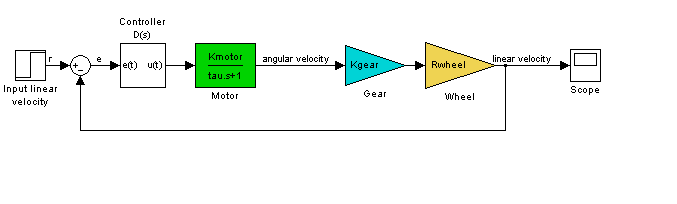
\includegraphics[width=0.8\textwidth]{resources/speed_blockdiagram}
	\caption{Block diagram of velocity control}
	\label{fig:control_1}
\end{figure}

\subsubsection{Position controller}

When a specific position is needed (counted as pulses from the encoders), another controller is used. This time the error signal is calculated as the difference between the actual position, and a given reference. Figure \ref{fig:control_2} shows a simplistic model of the position control feedback loop.

\begin{figure}[!ht]
	\centering
	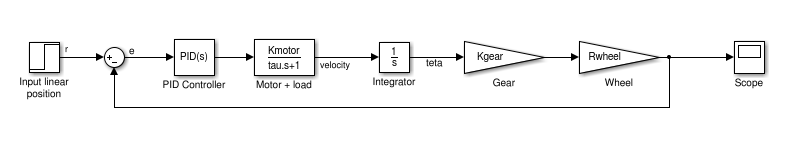
\includegraphics[width=0.8\textwidth]{resources/position_blockdiagram}
	\caption{Block diagram of position control}
	\label{fig:control_2}
\end{figure}

\subsubsection{Speed-position controller (straight forward)}

The last case for the motor controller, is to use a combination of the two above. In this controller, the error is a speed for each motor, but the error signal is calculated as both the difference between the reference speed and the actual speed, but also the difference in position between the two wheels. This ensured that both motors are driving at the same speed, hence a motor slows down or speeds up, to keep up with the other motor.

This controller is implemented as a more advanced PI-controller, to ensure that the steady-state error approaches zero. 

%
%
%
%
\subsection{Controllers in the Raspberry Pi}

\subsubsection{Following the line}
When following the line, a PID controller implemented in the Raspberry Pi, uses the camera as error signal, and calculates the necessary compensation. This compensation is a speed for the left and right motor, which are sent to the XMEGA motor controller over I2C. In the XMEGA a simple P-controller uses the speed received from the Raspberry Pi as 
a reference, and together with its encoder measurements, a speed for each motor is calculated.

\subsubsection{Following the wall}
Whenever the wall is to be followed, a special controller implemented in the Raspberry Pi is used. The error signal is calculated using the two distance sensors mounted on the left side of the robot.

\begin{equation}\label{eq:control_1}
	e = (d_s - d_1) + (d_2 - d_1)
\end{equation}

Equation \ref{eq:control_1} states that, the error is the difference between the front sensor and the desired reference (set point), plus the difference between the two sensors ($d_1$ and $d_2$). The first terms gives the an error if the robot is not the correct distance from the wall, where as the second term gives an error if the robot is not perfectly parallel with the wall.

%Keywords:  Controller, PID , Implementation, design, tuning, \citep{nise2011}, \citep{friesel_note7}, \citep{friesel_note9}

%
%
%
%
\section{Design of controllers}

\subsection{PID}
PID (proportional-integral-derivative) controller, also known as classical three-term controller, is a closed-loop feedback controller/compensator, widely used in the industry. An error signal is calculated as the difference between a desired `setpoint`, and an actual `process value`. Figure \ref{fug:control_3} illustrates a unity-feedback system with a PID-controller. 

\begin{figure}[!ht]
	\centering
	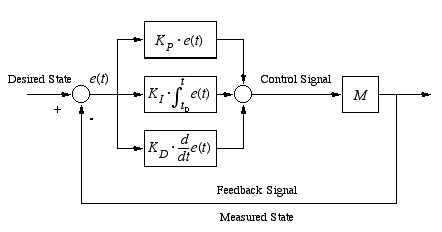
\includegraphics[width=0.5\textwidth]{resources/pid}
	\caption{PID Controller in feedback a feedback loop (from cs.brown.edu)}
	\label{fig:control_3}
\end{figure}

The figure shows each term of the PID-controller in time-domain. More often, it is more convenient to describe controllers and systems in frequency domain. The usual forms of the transfer function for a PID controller is given in equation \ref{eq:control_2}.

\begin{equation}\label{eq:control_2}
	D(s) = K_P + \frac{K_I}{s} + K_D s = \frac{K_Ds^2 + K_Ps + K_I}{s} = K_P(1 + \frac{1}{T_Is} + T_Ds)
\end{equation}

In chapter \ref{ch:simu}, we will look more into the actual parameters chosen for the controllers, and look at simulations and compare them against reality. 


%
%
%
%
\section{Implementation of discrete controller}

All controllers in the system are implemented in C using the reference implementation provided by Atmel, in their Application Note on Discrete PID controllers, \citep{avr221}, which again is based on theory by \citep{aastrom1995}.  

The argument `pid\_data\_t` is an abstract data type, with the fields needed by each calculation. It contains the P, I, D factors, the sum of error (for I-term), the last process value (for D-term), plus some other fields. 

\lstset{language=C,basicstyle=\tiny,numbers=left}
\begin{figure}
\begin{lstlisting}[frame=single,caption=Implementation of discrete PID controller,label=lst:control_1]
void pid_ctrl(pid_data_t * pid, int process_value)
{
	float p, i, d;
	float temp, cv;
	int error;

	error = pid->set_point - process_value;
	
	// Calculate P-term
	p = pid->P * error;

	// Calculate I-term
	pid->sum_error = pid->sum_error + error;
	if (pid->sum_error > pid->max_sum_error || pid->sum_error < -pid->max_sum_error)
	{
		pid->sum_error = 0;
	}
	i = pid->I * pid->sum_error;

	// Calculate D-term
	d = pid->D * (pid->last_process_value - process_value);
	pid->last_process_value = process_value;

	// Total correction (control variable)
	cv = p + i + d;
	if (pid->set_cv != NULL)
	{
		pid->set_cv(pid, cv);
	}
}
\end{lstlisting}
\end{figure}

%
%
%
%
\section{Tuning of PID controllers}

%Manual tuning, Ziegler-Nichols, Cohen-Coon

\subsection{Manual tuning}
The simplest of the known tuning methods, is called manual tuning \citep{zhong2006}. By starting with $K_P = 1$, $K_D = 0$, and $K_I = 0$, and then using the table below to tune the system. This method has been heavily used during this project.

\begin{table}
\begin{center}
\caption{Tuning parameters}
\begin{tabular}{| l | l | l | l | l |}
	\hline
	Response & Rise Time & Overshoot & Settling Time & S-S Error \\ \hline
	$K_P$ & Decrease & Increase & No change & Decrease \\ \hline
	$K_I$ & Decrease & Increase & Increase & Eliminate \\ \hline
	$K_D$ & No change & Decrease & Decrease & No change \\ \hline
\end{tabular}
\label{tbl:control_1}
\end{center}
\end{table}

From table \ref{tbl:control_1} we can conclude the following:

\begin{itemize}
	\item Use $K_P$ to increase rise time.
	\item Use $K_D$ to reduce the overshoot and settling time.
	\item Use $K_I$ to eliminate the steady-state error.
\end{itemize}

\subsection{Ziegler-Nichols}

Another important method for tuning PID-controllers is the Ziegler-Nichols method, which in the industry is accepted as standard \citep{copeland2008}. Ziegler and Nichols actually came up with two methods, but only their second method is given here. 

Tuning using Ziegler-Nichols second method requires the following steps (from \citep{copeland2008}):

\begin{itemize}
	\item Reduce the integrator and derivative gains to 0
	\item Increase $K_P$ to some critical value $K_{cr}$ at which sustained oscillations occur. 
	\item Note the value of $K_{cr}$, and the corresponding period of sustained oscillations, $P_{cr}$
\end{itemize}

The gains are now to be found using table \ref{tbl:control_2}.

\begin{table}
\begin{center}
\caption{Ziegler-Nichols - Second method}
\begin{tabular}{| l | l | l | l |}
	\hline
	PID Type & $K_P$ & $T_i$ & $T_d$ \\ \hline
	P & $0.5 K_{cr}$ & $\infty$ & 0 \\ \hline
	PI & $0.45 K_{cr}$ & $P_{cr}/1.2$ & 0 \\ \hline
	PID & $0.6 K_{cr}$ & $P_{cr}/2$ & $P_{cr}/8$ \\ \hline
\end{tabular}
\label{tbl:control_2}
\end{center}
\end{table}

